\section{Introduction}

The number of Internet of Things applications is forecast to exponentially grow within the coming decade. Owners of such applications strive to make predictions from large streams
of complex input in near real time. Cloud-based architectures often centralize storage and processing, generating high data movement overheads that penalize real-time applications. Edge and Cloud architecture pushes computation closer to where the data is generated, reducing the cost of data movements and improving the application response time. The heterogeneity among the edge devices and cloud servers introduces an important challenge for deciding how to split and orchestrate the IoT applications across the edge and the cloud. In this chapter, we propose a solution on how to split IoT applications dynamically across the edge and the cloud, allowing us to improve performance metrics such as end-to-end latency (response time), bandwidth consumption, and edge-to-cloud and cloud-to-edge messaging cost. 

\section{Problem Description}
We focus on three performance metrics for placing \ac{IoT} applications across edge and cloud resources, \textit{i.e.}, the end-to-end application latency~\cite{daSilvaVeith:2018}, the WAN traffic, and the messaging cost (messages exchanged between the edge and the cloud). The \ac{IoT} operator placement problem consists of defining how to accommodate the application components (\textit{i.e.}, operators) on the available resources of the network topology to optimize one or more performance metrics. 

Table~\ref{tab:symbology} summarizes the notation used throughout the paper.
\begin{table}[ht]
  \centering
  \caption{Main notation adopted for the problem description.}
  \label{tab:symbology}
  \begin{tabular}{ll}
    \toprule
    Symbol & Description\\
    \midrule
    $\mathcal{R}$ & Set of cloud and edge resources\\
    $\mathcal{L}$ & Set of network links\\
    $i\!\leftrightarrow\!j$ & A link connecting resources $i$ and $j$ \\
    $cpu^r_i$, $mem^r_i$ & CPU and memory capacities of resource $i$ \\
    $lat_{i\!\leftrightarrow\!j}$,$bdw_{i\!\leftrightarrow\!j}$ & Latency and bandwidth of link $i\!\leftrightarrow\!j$ \\
    $\mathcal{O}$ & Set of stream processing operators \\
    $\mathcal{S}$ & Set of event streams between operators \\
%     $\mathcal{O}^{src}$, $\mathcal{O}^{out}$, $\mathcal{O}^{trn}$ & Sources, sinks and transformations \\  
    $f_i$ & Function to determine if the operator is a source, sink \\
    & and transformation\\
    $cpu^o_i$, $mem^o_i$ & CPU and memory req. of operator $i$\\
    $\psi^o_i$ & Selectivity of operator $i$\\
    $\omega^o_i$ & Data compression rate of operator $i$\\
    $s^{\rho}_{i\rightarrow j}$ & Probability that a message emitted\\ 
    &  by operator $i$ will flow to $j$\\ 
    $\lambda_i^{in},\lambda_i^{out}$ & Input/output event rate of operator $i$\\
    $\varsigma_i^{in},\varsigma_i^{out}$ & Input/output event size of operator $i$\\
    $stime_{\langle i,k\rangle}$ & Service time of operator $i$ at resource $k$\\
    $ctime_{\langle i,k\rangle\langle j,l\rangle}$ & Communication time from operator $i$ \\ 
    & at resource $k$ to $j$ at $l$ \\
%     $\varphi^{comp}_{\langle i,k\rangle}$ & Event service time of operator $i$\\
%     & at resource $k$\\ 
    $mem_{\langle i,k\rangle}$ & Overall memory required by operator\\
    &  $i$ when deployed at resource $k$\\
    $p_i, l_{p_i}$ & A graph path and its end-to-end latency\\ 
    $\mathcal{P}$ & The set of all paths in an application graph\\
    $\mu_{\langle i,k\rangle}$ & The rate at which operator $i$ \\
    & can process events at resource $k$\\
    \bottomrule
\end{tabular} 
\end{table}


We define a computational resource (\textit{i.e.}, cloud server or edge device) as a triple $ r_k = \langle cpu_k^r, mem_k^r, f_k^r\rangle \in\mathcal{R}$, where $cpu_k^r$ is the CPU capability in \ac{MIPS}, $mem_k^r$ is the memory capability in bytes, and $f_k^r\in\{0, 1\}$ signals whether $r_k$ is a \textit{cloud} resource. Similarly, the network link is drawn as a triple $l_{k\leftrightarrow l}=\langle bdw_{k\leftrightarrow l},lat_{k\leftrightarrow l}, f_{k\leftrightarrow l}\rangle\in\mathcal{L}$, where $k\leftrightarrow l$ represents the interconnection between resource $k$ and $l$, $bdw_{k\leftrightarrow l}$ the bandwidth capability in bits per second (bps), $lat_{k\leftrightarrow l}$ the latency in seconds, and $f_{k\leftrightarrow l}$ signals whether the link is part of a WAN. We consider the latency of a resource $k$ to itself (\textit{i.e} $lat_{k\leftrightarrow k}$) to be $0$.  

Each operator of the \ac{IoT} application is a quintuple $o_i = \langle cpu_i^o, mem_i^o, \psi_i^o, \omega_i^o, f_i\rangle\in\mathcal{O}$, where $cpu_i^o$ is the CPU requirement in \ac{IPS} to handle an individual event, $mem_i^o$ is the memory requirement in bytes to load the operator, $\psi_i^o$ is the ratio of number of input events to output events (\emph{i.e.}, selectivity), $\omega_i^o$ is the ratio of the size of input events to the size of output events (\emph{i.e.}, data compression/expansion factor), and $f_i\in\{source,sink,transformation\}$ signals whether $o_i$ is a \textit{source}, \textit{sink/output}, or \textit{transformation}. The rate at which operator $i$ can process events at resource $k$ is denoted by $\mu_{\langle i,k\rangle}$ and is essentially $\mu_{\langle i,k\rangle} = cpu_k^r\div cpu_i^o$. An event stream $s_{k\rightarrow l}^{\rho}\in\mathcal{S}$ connects operator $k$ to $l$ with a probability $\rho$ that an output event emitted by $k$ will flow through to $l$.

\begin{figure}
  \centering
  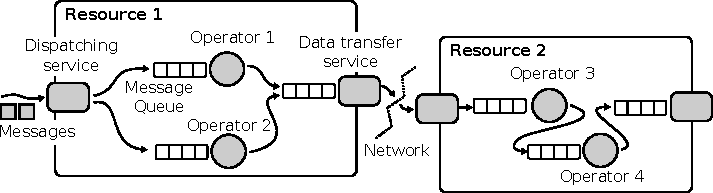
\includegraphics[width=1\columnwidth]{Figures/resource_model.pdf}
  \caption{Example of four operators and their respective queues placed on two resources.}
  \label{fig:deployment}
\end{figure}

The rate at which operator $i$ produces events is denoted by $\lambda_i^{out}$ and is a product of its input event rate $\lambda_i^{in}$ and its selectivity ($\psi^o_i$). The output event rate of a source operator ($f_k=source$) depends on the number of measurements it takes from a sensor or another monitored device. Likewise, we can recursively compute the average size $\varsigma_i^{in}$ of events that arrive at a downstream operator $i$ and the size of events it emits $\varsigma_i^{out}$ by considering the upstream operators' event sizes and their respective compression/expansion factors (\textit{i.e.}, $\omega^o_i$).

A computational resource can host one or more operators; operators within a same host communicate directly whereas inter-node communication is done via a communication service as depicted in Figure~\ref{fig:deployment}. Events are handled in a \ac{FCFS} fashion both by operators and the communication service that serialises messages to be sent to another host. Both operators and the communication service follow an M/M/1 model for their queues which allows for estimating the waiting and service times for computation and communication. The computation or service time $stime_{\langle o_i,r_k\rangle}$ of an operator $i$ placed on a resource $k$ is hence given by:

\begin{equation}
stime_{\langle i,k\rangle} = \frac{1}{\mu_{\langle i,k\rangle} - \lambda_{i}^{in}}
\label{eq:computation}
\end{equation}

\noindent while the communication time $ctime_{\langle i,k\rangle\langle j,l\rangle}$ for operator $i$ placed on a resource $k$ to send a message to operator $j$ on a resource $l$ is:
\begin{equation}
ctime_{\langle i,k\rangle\langle j,l\rangle} = \frac{1}{\Big(\frac{bdw_{k\leftrightarrow l}}{\varsigma_{i}^{out}}\Big) - \lambda_{j}^{in}} + l_{k\leftrightarrow l}
\label{eq:communication}
\end{equation}

A mapping function $\mathcal{M} : \mathcal{O} \rightarrow \mathcal{R}$, $\mathcal{S} \rightarrow \mathcal{L}$ indicates the resource to which an operator is assigned and the link(s) to which a stream is mapped. The function $mo_{\langle i,k\rangle}$ returns $1$ if operator $i$ is placed on resource $k$ and $0$ otherwise. Likewise, the function $ms_{\langle i\rightarrow j,k\leftrightarrow l\rangle}$ returns $1$ when the stream between operators $i$ and $j$ has been assigned to the link between resources $k$ and $l$, and $0$ otherwise.

A \textit{path} in the \ac{IoT} application graph is a sequence of operators from a source to a sink. A path $p_i$ of length $n$ is a sequence of $n$ operators and $n-1$ streams, starting at a source and ending at a sink:
\begin{equation}
p_i = o_{0},o_{1},\dots,o_{k},o_{k+1},\dots,o_{n-1}, o_{n} 
\end{equation}
  
Where $o_0=source$ and $o_n=sink$. The set of all possible paths in the application graph is denoted by $\mathcal{P}$. The end-to-end latency of a path comprises the sum of the computation time of all operators along the path and the communication time required to stream events on the path. More formally, the end-to-end latency of path $p_i$, denoted by $L_{p_i}$, is:


\begin{equation} \label{eq:latency}
  \begin{split}
  L_{p_i} =
  \sum_{\substack{o\in \mathcal{O} \\
                  r\in\mathcal{R}
                 }
        } 
   mo_{\langle o,r\rangle} \times stime_{\langle o,r\rangle} \\
   + \sum_{\substack{r'\in\mathcal{R}
                    }
         }    
   ms_{\langle o\rightarrow o+1,r\leftrightarrow r'\rangle} \times ctime_{\langle o, r\rangle\langle o+1,r'\rangle}      
  \end{split}   
\end{equation}

The WAN traffic accumulates the sizes of messages that cross the WAN network where $\mathbb{1}_{\{f_{k\leftrightarrow l} = 1\}}$ is the indicator that the link between the resource $k$ and $l$ is on a WAN. The WAN traffic of path $p_i$ is calculated as:
\begin{equation}
      W_{p_i} = \sum\limits_{
 \substack{s_{i\rightarrow j}\in\mathcal{S}\\
 k \leftrightarrow l\in\mathcal{L}
 }
 }{
    \mathbb{1}_{\{f_{k\leftrightarrow l} = 1\} } \times ms_{\langle i\rightarrow j,k\leftrightarrow l\rangle} \times \varsigma_i^{out}\quad 
 }
  \label{eq:traffic}
\end{equation}

Likewise, the messaging cost is calculated by the number of messages that reaches the cloud from the edge and vice versa. The indicator $\mathbb{1}_{ \{f_{k}^{r}=0\text{ and }f_{k^\prime}^{r} = 1\}}$ indicates that the previous operator $i$ is placed on edge ($f_{k}^r=0$) and it sends messages to operator $i^\prime$ in cloud ($f_{k^\prime}^{r} = 1$), the second part of the cost refers the other way cost (cloud to edge). The number of messages in $p_i$ is given as:
\begin{equation}
  \begin{split} 
    C_{p_i} = \smash{\sum_{\substack{i\in \mathcal{O} \\
                  i^\prime\in \mathcal{O} \\
                  k\in\mathcal{R} \\
                  k^\prime\in\mathcal{R}
                 }
          }      }
        \Big(\mathbb{1}_{ \{f_{k}^{r}=0\text{ and }f_{k^\prime}^{r} = 1\}}\times \big(mo_{\langle i^\prime,k^\prime\rangle} \times \\ \lambda_{i^\prime}^{in} + mo_{\langle i, k\rangle} \times\lambda_{i^\prime}^{out}\big) \Big)
  \end{split} 
  \label{eq:cost}
\end{equation}
\\

The parameters latency ($Par_{lat}$), WAN traffic ($Par_{wan}$), and monetary cost ($Par_{cost}$) receive the current values of the running application. A single aggregate cost metric uses the parameters and \textit{Simple Additive Weighting method} \cite{yoon:1995} (normalized in the interval [0,1]) offers a unified metric where $w_l$, $w_w$ and $w_c$, with $w_l + w_w + w_c = 1$, are non-negative weights for the different costs. Each metric of path $p_i$ is divided by its corresponding parameters and is then multiplied by its weight. The sum of the three metrics in the path $p_i$ results in the aggregate cost. Formally, the $AggregateCost$ in $p_i$ is determined as:


\begin{equation}
  \begin{split} 
    AggregateCost_{p_i} = w_l\times \frac{L_{p_i}}{Par_{lat}} + \\ w_w\times\frac{W_{p_i}}{Par_{wan}}+ w_c\times\frac{C_{p_i}}{Par_{cost}}
  \end{split}    
  \label{eq:placement}
\end{equation}

The problem of placing a distributed \ac{IoT} application consists of finding a mapping that minimizes the aggregate cost. % of all application paths and that respects the resource and network constraints. In other words, find the mapping that minimises the aggregate end-to-end event latency:

\begin{equation}
  \min \sum\limits_{p_i\in\mathcal{P}}{AggregateCost_{p_i}}
  \label{eq:objectivefunction}
\end{equation}
Subject to:
\begin{equation}
  \lambda_{o}^{in} < \mu_{\langle o,r\rangle} \quad\quad \forall o\in\mathcal{O}, \forall r\in\mathcal{R} | mo_{\langle o,r\rangle} = 1  
  \label{eq:comp_staturation}
\end{equation}
\begin{equation}
  \lambda_{o}^{in}<\Big(\frac{bdw_{k\leftrightarrow n}}{\varsigma_{o-1}^{out}}\Big) \quad\quad  \forall o\in\mathcal{O}, \forall k\!\leftrightarrow\!n\in\mathcal{L} |  mo_{\langle o,k\rangle} = 1 
    \label{eq:comm_staturation}
\end{equation}
\begin{equation}
 \sum_{o\in\mathcal{O}}mo_{\langle o,r\rangle}\times\lambda_{o}^{in} \le cpu_r \quad\quad \forall r\in\mathcal{R}
  \label{eq:comp_av}
\end{equation}
\begin{equation}
\sum _{o \in \mathcal{O}}
{
mo_{\langle o,r\rangle} \times mem_{\langle o,r\rangle} \le mem_{r} \quad\quad \forall r\in\mathcal{R}
}
   \label{eq:mem_av}
\end{equation}
\begin{equation}
 \sum\limits_{
 \substack{s_{i\rightarrow j}\in\mathcal{S}\\
 k \leftrightarrow l\in\mathcal{L}
 }
 }{
    ms_{\langle i\rightarrow j,k\leftrightarrow l\rangle} \times \varsigma_i^{out} \le bwd_{k \leftrightarrow l} \quad\quad \forall k \leftrightarrow l\in\mathcal{L}
 }
   \label{eq:comm_av}
\end{equation}
\begin{equation}
 \displaystyle \sum _{r \in \mathcal{R}} mo_{\langle o,r\rangle} = 1 \quad\quad \forall o \in \mathcal{O}
 \label{eq:vertex_map}
\end{equation}
\begin{equation}
 \sum\limits_{
 \substack{
%  s_{i\rightarrow j} \in \mathcal{S}\\
 k\leftrightarrow l \in \mathcal{L}}}
 {
 ms_{\langle i\rightarrow j,k\leftrightarrow l\rangle} = 1 \quad\quad \forall s_{i\rightarrow j} \in \mathcal{S}
 }
  \label{eq:edge_map}
\end{equation}

Constraint \ref{eq:comp_staturation} guarantees that a resource can provide the service rate required by its hosted operators whereas Constraint \ref{eq:comm_staturation} ensures that the links are not saturated. The CPU and memory requirements of operators on each host are ensured by Constraints~\ref{eq:comp_av} and \ref{eq:mem_av} respectively. Constraint~\ref{eq:comm_av} guarantees the data requirements of streams placed on links. Constraints \ref{eq:vertex_map} and \ref{eq:edge_map} ensure that an operator is not placed on more than a resource and that a stream is not placed on more than a network link respectively.

\section{R-Pulsar Framework Extension}\label{sec:framework}
R-Pulsar is a data analytics software stack for collecting, processing, and analyzing data at the edge and/or at the cloud. R-Pulsar has been extended to allow developers the ability to decide \textbf{how} to split the application operators between the edge and the cloud, by specifying a set of constraints. 

R-Pulsar consists of the associative rendezvous programming model (AR), an abstraction for content-based decoupled interactions (interactions defined in terms of semantic profiles instead of names) and rendezvous points~\cite{Renart2018EdgeBD}. The rendezvous point (RP) is a node where the dataflow computations occur, and it can be a gateway located at the edge of the network or a server in the cloud. R-Pulsar uses a peer-to-peer (P2P) network to connect and communicate with all the RP nodes. 

\subsection{R-Pulsar Layers}
R-Pulsar has been extended with the following three layers in order to automatically split and orchestrate dataflows between the edge and the cloud. 

\textbf{R-Pulsar Infrastructure Controller:} Designed to act similarly to software-defined networking (SDN) controllers, this layer keeps track of the network resources available in real time. Some of the basic tasks include inventorying devices within the R-Pulsar P2P network, their capabilities, locations, and network statistics.

\textbf{R-Pulsar Plan Finder:} This layer computes the most optimized operator placement plan. It uses a three-step approach for calculating the optimal operator placement plan for deploying dataflows between the edge and the cloud. Section~\ref{sec:strategies} presents the three-step operator placement strategy developed for R-Pulsar.

\textbf{R-Pulsar Executor/Monitor:} The primary responsibility is to monitor dataflows running on the R-Pulsar P2P network, including dataflow deployment, task assignment, and task reassignment in case of failure.

\subsection{R-Pulsar Nodes}

Each rendezvous point (RP) in the R-Pulsar P2P network can be elected as a master or as a worker. R-Pulsar differs from other master/slave clusters such as Apache Storm~\cite{storm} in the sense that R-Pulsar master and worker node roles are assigned dynamically every time a dataflow is deployed. 
\\\\
\textbf{Master RP:}
The master RP's primary responsibility is to manage, coordinate, and monitor a dataflow running on the R-Pulsar P2P network, including dataflow deployment, task assignment, and task reassignment in the event of a failure. Each time a new dataflow is deployed in the P2P network a new master RP for that dataflow is elected.

Deploying a topology to the R-Pulsar P2P network involves submitting the pre-packaged dataflow file along with topology configuration. Then the information will be routed to the responsible RP using the content-based interactions~\cite{Renart2018EdgeBD}. The content-based interactions allow users to route dataflows to unknown RPs; the RP who receives the message will be automatically elected as the master RP for that dataflow. Once the master RP has been elected, it then uses the infrastructure controller layer to collect the network information of all the worker RPs. That information is then passed to the operator placement algorithm to generate a placement strategy. Once the operator placement algorithm has an efficient operator placement plan, then the master RP distributes the tasks to the worker RPs.

The master RP tracks the status of all worker nodes and the tasks assigned to each one. If the master RP detects that a specific worker node has failed to heartbeat or has become unavailable, it will reassign that worker RP tasks to other worker RP nodes in the federation.

The master RP is not a single point of failure in the strictest sense. This quality is because the master RP does not take part in the dataflow data processing, rather it merely manages the deployment, task assignment, and monitoring of the dataflow. In fact, if the master RP dies while a dataflow will continue to process data as long as the worker RPs assigned with tasks remain healthy. 

\textbf{Worker RP:} Each worker node is responsible for creating, starting, and stopping worker tasks assigned to that node. Worker RPs are also responsible for once the master RP has died to perform a master RP election.

\subsection{Placement Strategy}\label{sec:strategies}
The strategy for operator placement on R-Pulsar applies statistics collected by profiling the application and the location of sinks and sources. The operator placement aims to minimize the \textit{AggregateCost} (Equation~\ref{eq:objectivefunction}) by splitting the IoT application across edge and cloud by considering priorities of operators according to the infrastructure to which the sinks are assigned.
The operator placement strategy comprises three phases: (i) application profiling; (ii) candidate placement and (iii) final placement. 

\textbf{Phase 1 -- Application Profiling:}. 
In the first phase the worker RPs and the master RPs using the infrastructure controller layer continuously collect statistics~\cite{kaur:2017} from the running dataflow. The collected data includes the following information about the operators:
\begin{itemize}
  \item The arrival rate of events.
  \item Processing time per event.
  \item Number of MIPS required to process a tuple.
  \item Memory to run the operator.
  \item Arrival message size.
  \item Outcome message size.
\end{itemize}
This information is used to establish the selectivity, data compression/expansion factor, as well as, the CPU and memory requirements. 
\\
\\
\textbf{Phase 2 -- Candidate Placement:}
In phase two, the user-predefined locations of sinks and sources are used to identify patterns in the dataflow (Section~\ref{sec:api}). As depicted in Figure~\ref{fig:graph}, a dataflow can comprise multiple patterns such as (i) forks, where messages can be replicated to multiple downstream operators or scheduled to downstream operators in a round-robin fashion, using message key hashes, or considering other criteria \cite{Ni:2017}; (ii) parallel regions that perform the same operations over different sets of messages or where each individual region executes a given set of operations over replicas of the incoming messages; and (iii) joins, which merge the outcome of parallel regions. 

\begin{figure} 
  \centering
  \includegraphics[width=1\columnwidth]{Figures/patterns.pdf}
  \caption{Phases to determine the final placement using split points, where red means placed on edge, blue represents placed on cloud, and green delimits forks and joins.}
  \label{fig:graph}
\end{figure}

We consider that an IoT dataflow is a Series-Parallel-Decomposable Graph which either consists of a series of linearly dependent operators, or operators that can be executed independently in parallel, or a combination thereof. Phase 2 uses related techniques to identify graph regions that present these patterns \cite{Eidenbenz:2016}. This information is used to build a hierarchy of region dependencies (\textit{i.e.} downstream and upstream relations between regions) and assist in placing operators across cloud and edge resources. The streams in the graph paths that separate the operators are hereafter called the \textit{split points}. The rationale behind building such region hierarchy is to evaluate first the operators that can have greater impact on the overall end-to-end latency. Figure~\ref{fig:graph} illustrates the phases of the method to determine the split points (green circles), where red circles represent operators placed on edge resources whereas blue ones are on the cloud: (i) The method starts with sources and sinks whose placements are predefined by the user; (ii) split points are discovered (green circles) as well as sinks that correspond to actuators that can be placed on the edge; (iii) the branches between the existing patterns (green, red, and blue circles) are transformed into series regions; (iv) a hierarchy following the dependencies between regions is created; and (v) the regions provide information to split the operators on edge candidate placement evaluating if the operator flows events to actuators.

Algorithm~\ref{alg:patterns} describes the function $GetCandidates$ used to identify the patterns and obtain the series regions. First, the function adds two virtual vertices to the graph: $virt\_src$ connected to all data sources and $virt\_sink$ to which all sinks are connected (line~\ref{alg:patterns_virt_start}-\ref{alg:patterns_virt_end}). These vertices allow for recognizing all paths between sources and sinks. Second, each path is iterated moving operators to a temporary vector and classifying them as upstream and downstream according to the number of input and output edges (lines~\ref{alg:seriesregions_opdegree_begin}-\ref{alg:seriesregions_opdegree_downstream}). If the operator is a split point, the temporary vector is converted into a subset of regions set, and the temporary vector receives the current operator (lines~\ref{alg:seriesregions_opdegree_split}-\ref{alg:seriesregions_opdegree_addregions}). Third, the function removes the redundant values (line~\ref{alg:seriesregions_delete}). Fourth, the region set is iterated comparing the regions by the first and the last position values (equal values represent a connection) and consequently, they are stored in the hierarchy set (lines~\ref{alg:seriesregions_series_start}-\ref{alg:seriesregions_series_hier}). At last, using the hierarchy and the placement of the sinks, the function evaluates if the operator flows events to sinks placed on edge device then the operators is added to the $candidate$ lines~\ref{alg:begin_candidate_placement}-\ref{alg:end_candidate_placement}). 

\IncMargin{-0.4em} 
\RestyleAlgo{ruled}\LinesNumbered
\newcommand{\rand}{\emph{\textbf{and}}\xspace}
\newcommand{\ror}{\emph{\textbf{or}}\xspace}
\begin{algorithm}[ht]
\caption{Algorithm to get the candidate placement.}
\label{alg:patterns}
\DontPrintSemicolon
\SetAlgoLined
\SetAlgoVlined
\SetKwFunction{GetAllPaths}{GetAllPaths}
\SetKwFunction{SeriesRegions}{SeriesRegions}
\SetKwFunction{GetSinks}{GetSinks}
\SetKwFunction{GetLocation}{GetLocation}
\SetKwFunction{Break}{Break}
\SetKwProg{Fn}{Function}{}{}

\Fn{GetCandidates($\mathcal{G} = (\mathcal{O},\mathcal{S})$)}{
   $\mathcal{O} \gets \mathcal{O}\cup virt\_src\cup virt\_sink$\label{alg:patterns_virt_start}\; 

%    \For{$o\in \mathcal{O}^{src}$}{
      $\mathcal{S} \gets \mathcal{S} \cup s_{virt\_src \rightarrow o}, \forall o\in\mathcal{O}\text{ and } f_o=\text{source}$\;                       
%    }
%    $\mathcal{O} \gets \mathcal{O}\cup virt\_sink$\;
%    \For{$o\in \mathcal{O}^{out}$}{
      $\mathcal{S} \gets \mathcal{S} \cup s_{o \rightarrow virt\_sink}, \forall o\in\mathcal{O}\text{ and } f_o=\text{sink}$\label{alg:patterns_virt_end}\;  
%    }
%    $paths \gets $ \GetAllPaths{$\mathcal{G}, virt\_src, virt\_sink$}\label{alg:patterns_paths}\;
   
   
   
  %$temp \gets \{\}, regions \gets \{\}, hierarchy \gets \{\}$\label{alg:seriesregions_opdegree_start}\;
  \For{$p \in\text{ }$\GetAllPaths{$\mathcal{G}, virt\_src, virt\_sink$}}{\label{alg:seriesregions_opdegree_begin}
     \For{$o \in p$}{
%         \If{$(o\neq virt\_src$ \rand $o\neq virt\_sink)$}{
          $temp \gets temp\cup\{o\}, \forall o\not\in\{virt\_src,virt\_sink\}$\label{alg:seriesregions_opdegree_store}\;
%         }        
        $ups \gets |\langle *,o\rangle\subset\mathcal{S}|, downs \gets |\langle o,*\rangle\subset\mathcal{S}|$\label{alg:seriesregions_opdegree_downstream}\;
        
        \If{$ups >1$ \ror $downs >1$ \rand $ o\not\in\{virt\_src,virt\_sink\}$}{\label{alg:seriesregions_opdegree_split}
%           \If{$o \neq virt\_src$ \rand $o\neq virt\_sink $}{
              $regions \gets regions \cup temp,$ $temp \gets \{o\}$\label{alg:seriesregions_opdegree_addregions}\;
        %      $temp \gets \{o\}$\label{alg:seriesregions_opdegree_end}\;
%           }
        }
     }
  }
  Delete duplicate $regions$\label{alg:seriesregions_delete}\;
  \For{$src \in regions$}{\label{alg:seriesregions_series_start}
     \For{$dst \in regions$}{
        \If{$src \neq dst$}{\label{alg:seriesregions_series_end}
          \If{$src[|src|-1] = dst[0]$}{
             $hierarchy \gets hierarchy \cup \{src, dst\}$\label{alg:seriesregions_series_hier}\;
          }
        }
     }
  }
  
  
  \For{$operators \in regions$}{\label{alg:begin_candidate_placement}
     \For{$o \in operators$}{
       \If{$f_o\not\in\{source,sink\}$}{
          \For{$sink \in \GetSinks{$o$}$}{
            \If{\GetLocation{$sink$} = $edge$}{
              $candidate=candidate\cup o$\;
              \Break\; \label{alg:end_candidate_placement}
            }      
          }
       }  
    }
  }
  
    
  
  \Return{$candidate$}
}

\end{algorithm}

\textbf{Phase 3 -- Final Placement:} 
Once phase two has completed and the profiling phase has established the requirements from the different operators, an operator placement strategy is created and deployed. The strategy reduces the combinatorial space by estimating only once the computation (Equation~\ref{eq:computation}) and communication (Equation~\ref{eq:communication}) overheads to operators targeted to cloud (Phase 2). Otherwise, operators to edge (edge candiate placements) have their overheads estimated for all edge devices evaluating their constraints (Equation~\ref{eq:comp_staturation} --~Equation~\ref{eq:edge_map}). The strategy gives high priority to edge since cloud sinks often store messages for batch processing, whereas the edge side hosts actuators.
If edge devices cannot meet all operator requirements then the operator is moved to the cloud, hence, the cloud hosts its operator candidates and those that do not meet the constraints on edge. For instance, Operator 5 in Figure~\ref{fig:graph} was reallocated since the edge does not respect the resource constraints. Along with the overhead estimations, the strategy greedly uses the edge candiate placements for sequentially estimating the $AggregateCost$ (Equation~\ref{eq:placement}) and at each iteration, it picks the device with the minimal value (Equation~\ref{eq:objectivefunction}) to assign the operator.

\subsection{R-Pulsar API}
\label{sec:api}
In this section we present the API examples used for evaluating and deciding \textbf{how} to split the ETL dataflow, between the edge and the cloud resources. 

Listing~\ref{lst:place} is for specifying the operator constraints. In our case some of the operators need to be placed at the cloud and some others need to be placed at the edge. Note that if the wildcard or no placement is specified R-Pulsar will automatically decide the best placement for the operator. CloudTableInsert, MQTTPublish, and BloomFilterTask are tasks used in the ETL dataflow.

\begin{lstlisting}[ caption={User specified operator physical placements constraints.}, captionpos=b, label={lst:place}]
op1.map(CloudTableInsert()).placement(cloud);
op2.map(MQTTPublish()).placement(edge);
op3.map(BloomFilterTask()).placement(*);
\end{lstlisting}

Listing~\ref{lst:method} is for specifying the optimizations to apply to the dataflow. The R-Pulsar operator placement algorithm offers three optimizations: minimize end-to-end latency, bandwidth, or messaging cost. Each of the functions requires a weight normalized in the interval [0,1]; the sum of all three weights must be one. By doing so, users have the ability to optimize the latency, data transfer rate and messaging cost at the same time.

\begin{lstlisting}[caption={User specified dataflow optimizations (latency, data transfer rate and cost).}, captionpos=b, label={lst:method}]
topology.minEndToEndLatency(0.4);
topology.minDataTransferRate(0.3);
topology.minMessagingCost(0.3);
\end{lstlisting}

By specifying physical dataflow constraints and the optimizations desired R-Pulsar can obtain an optimal operator placement plan.  

\section{Evaluation}\label{sec:evaluation}
This section presents an experimental evaluation of our system. First, we present the setup and the other approaches in which the experiments will be evaluated and compared against. Second, we present an evaluation of our system based on latency, data transfer rate, and messaging cost. 

\subsection{Setup}

Our experiments are performed using the following edge and cloud setup:

\begin{itemize}

\item We used an experimental edge testbed developed by the authors, inspired by Hu \textit{et. al.}~\cite{Hu2016QuantifyingTI} that consists of 13 Raspberry Pis; 5 Raspberry Pis model 3 (4x ARM Cortex-A53 1.2GHz, 1GB of RAM and 10/100 Ethernet), and 8 Raspberry Pis model 2 (4x ARM Cortex-A7 900MHz, 1GB of RAM and 100 Ethernet). 

\item For the cloud we used the Chameleon cloud~\cite{chameleon} with 5
instances of type m1.medium (2 CPU and 4 GB RAM).

\end{itemize}

The 13 Raspberry Pis are connected to the same LAN. The Raspberry Pis use the external WAN~\cite{Ha:2013} (the Internet) for connecting to cloud. The LAN has a latency 0.523 ms and a bandwidth of 15 Mbits/sec. The WAN has latency 66.75 ms, and bandwidth of 87.0 Mbits/sec.

In addition to the setup, each of our experiments is evaluated using three other strategies. We compared our system with the following approaches:

\begin{itemize}	
\item \textbf{Cloud:} deploys all operators in the cloud, apart from operators provided in the initial placement.

\item \textbf{LB (Taneja et. al.~\cite{Taneja:2017}):} iterate a vector containing the application operators, gets the middle host of the computational vector, and evaluates CPU, memory, and bandwidth constraints to obtain the operator placement.

\item \textbf{Random:} simulates the user trying to guess the best placement for the dataflow between the edge and the cloud. Random is the average of 15 different dataflow deployments between the edge and the cloud resources.
\end{itemize}

All the tests are evaluated using the ETL dataflow. The ETL dataflow is an implementation of the ETL RIoTBench topology, it consists of: a single data source outputting data every 5 seconds, 2 sinks one located at the edge and one located at the cloud, and 7 tasks that need to be deployed between the edge and the cloud of the network. The experiments were conducted using Sense Your City dataset\footnote{http://map.datacanvas.org} which consists of transmitting data each minute from sensors in 7 cities across 3 continents, with about 12 sensors per city. The data content includes metadata on the sensor ID, geolocation, and five timestamped observations (outdoor temperature, humidity, ambient light, dust, and air quality).
\subsection{End-to-end Tuple Latency Evaluation}

The end-to-end tuple latency corresponds to the sum of the mean times from the two paths in ETL dataflow (cloud and edge). The conducted experiment evaluates the end-to-end tuple latency using Equation~\ref{eq:placement} where $w_l$ is equal to 1, and $w_w$ and $w_c$ are equal to 0. The experiment aims to evaluate how efficient the cloud, Random, and LB approaches are at minimizing the end-to-end tuple latency and compare the R-Pulsar operator placement approach. In addition, three failures were manually injected to showcase the dynamicity and flexibility to recover from node failures. The first failure makes 38\% of the edge cluster unavailable (100 ms). The second failure affects the remaining 62\% of the nodes (300 ms). Before the 62\% of the nodes fail, the 38\% of the nodes are back online. The third and last failure affects 50\% of the cloud instances (505 ms).

\begin{figure}[h!]
  \centering
  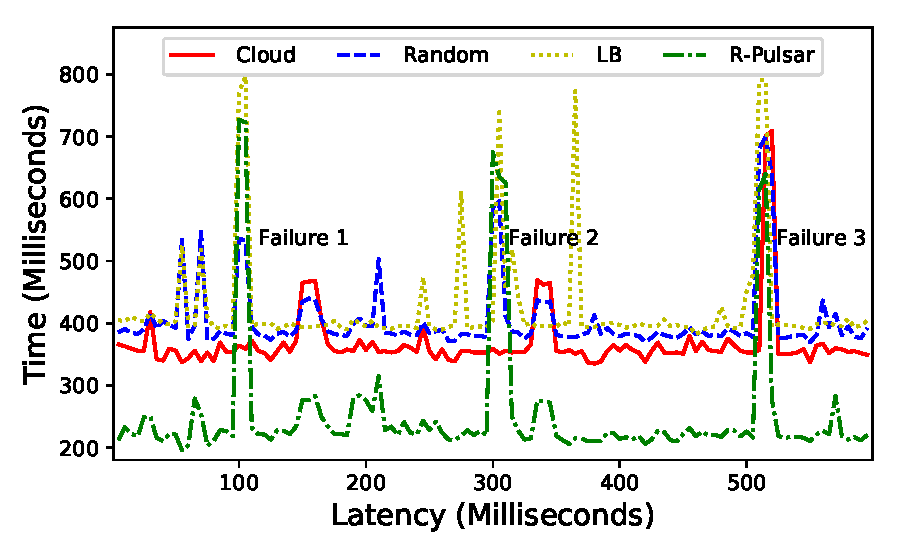
\includegraphics[width=0.8\textwidth]{Results/Latency.pdf}
  \caption{End-to-end tuple latency optimization with 3 self injected failures affecting edge and cloud nodes, while comparing it with Cloud, Random and LB approaches.}
  \label{fig:latency}
\end{figure} 

% \vspace{-2ex}

Figure~\ref{fig:latency} shows that on average tuples are computed 31\% faster when compared to the traditional cloud setup, and 38\% faster than Random and the LB placement approaches. The reason why the Random failures recover much faster than LB when compared to R-Pulsar is because Random is the average of multiple different deployments and in some cases the first failure is not affected. Figure~\ref{fig:latency} demonstrates that R-Pulsar operator placement strategy is capable of splitting the dataflow efficiently between the edge and the cloud and reduce the end-to-end tuple latency.

The second experiment aims to evaluate how efficient the Cloud, Random, and LB approaches are at minimizing end-to-end tuple latency and compare it with R-Pulsar approach. In this experiment no failures were injected.

\begin{figure}[h!]
  \centering
  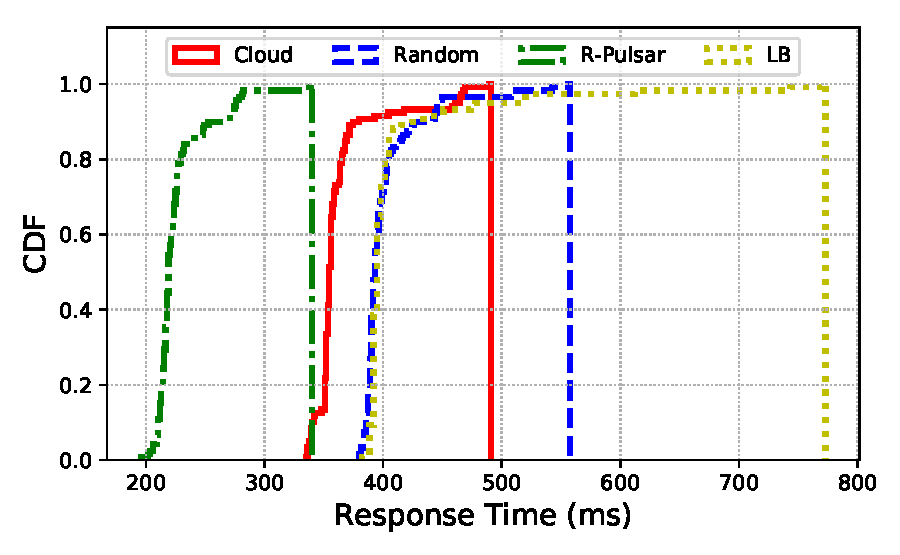
\includegraphics[width=0.8\textwidth]{Results/CDF_latency.pdf}
  \caption{End-to-end tuple latency optimization cumulative distribution function (CDF) comparison with Cloud, Random and LB approaches.}
  \label{fig:CDFLatency}
\end{figure} 

Figure~\ref{fig:CDFLatency} shows that when R-Pulsar operator placement approach is used 80\% of the tuples see a reduction in the end-to-end tuple latency by 44\% compared to the LB and Random approaches and 38\% compared to the cloud approach. 
 %R-Pulsar reduces the data transfers between the edge and the cloud by splitting the IoT application dataflow and by assigning operators to hosts to promote a better communication between themselves.

\subsection{Data Transfer Rate Evaluation}

The Data transfer rate consists of the sum of all message sizes that traverse a WAN link per second. The values for Equation~\ref{eq:placement} are $w_w$ equal to 1, and $w_l$ and $w_c$ equal to 0. This third experiment aims to evaluate how efficient are the cloud, Random, and LB approaches at minimizing the transfer rate between the edge and the cloud and compare the results with R-Pulsar operator placement approach. Minimizing the transfer rate between the edge and the cloud is a critical point in order to achieve real-time analytics. 

\begin{figure}
  \centering
  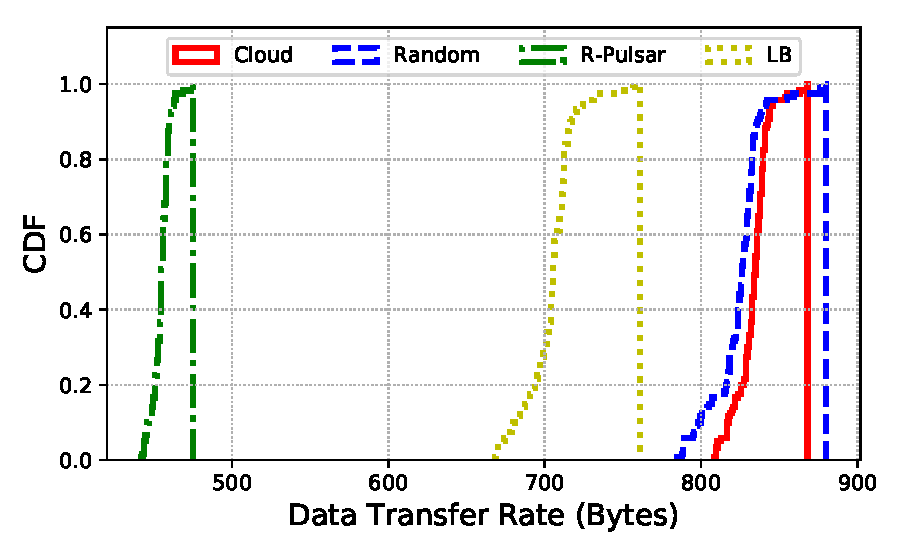
\includegraphics[width=0.8\textwidth]{Results/CDF_bandwidth.pdf}
  \caption{End-to-end data transfer rate optimization cumulative distribution function (CDF) comparison with cloud, Random and LB approaches.}
  \label{fig:bandwidth}
\end{figure} 


Figure~\ref{fig:bandwidth} shows that 80\% of the time R-Pulsar reduces the transfer rate between the edge and the cloud on average 35\% when compared to the LB approach. And it reduces the data transfer rate by 45\% when compared to the cloud and Random approaches.

This next experiment aims to evaluate the efficiency of minimizing the transfer rate and the end-to-end latency at the same time ($w_w$ = .5, $w_l$ = .5, and $w_c$ = 0). This experiment was also carried out using the cloud, Random, and LB approaches.

\begin{figure}
  \centering
  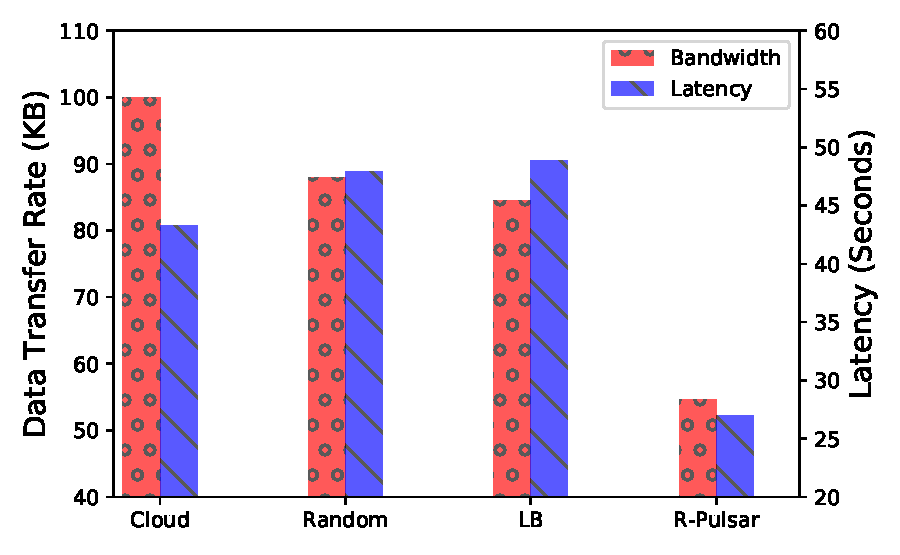
\includegraphics[width=0.8\textwidth]{Results/LandB.pdf}
  \caption{Multi optimization evaluation, end-to-end tuple latency and data transfer rate comparison with cloud, Random, and LB approaches.}
  \label{fig:both}
\end{figure} 

Figure~\ref{fig:both} shows that the R-Pulsar operator placement approach can also optimize the data transfer rate and the end-to-end latency by 46\% and 38\% respectively when compared to the cloud, 36\% and 45\% respectively when compared to the LB, 38\% and 44\% respectively when compared to the Random approach.

\subsection{Messaging Cost Evaluation}

The last two experiments aim to calculate the messaging cost of running the dataflow for a month using the cost models of two major actors, AWS and Microsoft, in a real life edge and cloud scenario. For this reason, we setup Equation~\ref{eq:placement} with $w_c$ equal to 1, and $w_l$ and $w_l$ equal to 0. The goal of this optimization is to reduce the number of messages that reach the cloud servers.

\begin{table}[h]
\caption{Azure IoT Hub and Amazon IoT Core messaging pricing.} \label{tb:table}
\centering
\begin{tabular}{cc}
\toprule
Microsoft IoT Hub Pricing                                                               & AWS IoT Core Pricing                                                              \\ \toprule
\begin{tabular}[c]{@{}c@{}}Free Tier - 8,000 messages/day\\ \$0\end{tabular}        & \begin{tabular}[c]{@{}c@{}}Every 1 million messages/day\\ \$1.00\end{tabular} \\ \hline
\begin{tabular}[c]{@{}c@{}}Tier 1- 400,000 messages/day\\  \$25\end{tabular}        & \begin{tabular}[c]{@{}c@{}}Up to 1 billion messages/day\\ \$1.00\end{tabular} \\ \hline
\begin{tabular}[c]{@{}c@{}}Tier 2 - 6,000,000 messages/day \\  \$250\end{tabular}   & \begin{tabular}[c]{@{}c@{}}Next 4 billion messages/day\\ \$0.80\end{tabular}  \\ \hline
\begin{tabular}[c]{@{}c@{}}Tier 3 - 300,000,000 messages/day\\ \$2,500\end{tabular} & \begin{tabular}[c]{@{}c@{}}Over 5 billion messages/day\\ \$0.70\end{tabular}  \\ \bottomrule
\end{tabular}
\end{table}

Table~\ref{tb:table} depicts two IoT cost models. The first cost model is the Microsoft Azure IoT Hub~\cite{HubPricing}. Each tier enables a maximum number of messages exchanged between the Azure IoT Edge and the Azure IoT Hub and vice versa per day. T1 allows up to 400,000 messages a day, T2 allows up to 6,000,000 messages a day, and T3 allows up to 300,000,000 messages a day. 

The second cost model is the Amazon IoT Core~\cite{AWSPricing} where messaging is metered by the number of messages transmitted between your devices and AWS IoT Core and vice versa per day. Amazon offers multiple costs for different regions, for this experiment we choose the cheapest region (N.Virginia) which charges \$1 per million messages sent, and the cost per message decreases after the first 1 billion messages per day.

\begin{figure}[h!]
  \centering
  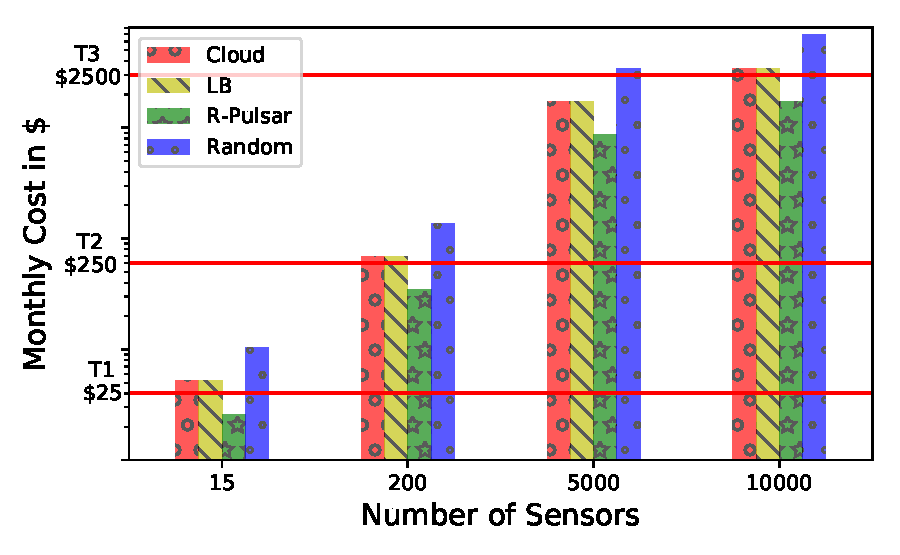
\includegraphics[width=0.8\textwidth]{Results/Cost_Microsoft.pdf}
  \caption{Messaging cost savings evaluation based on the Microsoft Azure IoT Hub pricing model, for four different setups.}
  \label{fig:cost-microsoft}
\end{figure} 

% \vspace{-2ex}

Figure~\ref{fig:cost-microsoft} depicts the cost of deploying the ETL dataflow using the Microsoft cost model using the four different approaches presented earlier. When using a small setup (15 sensors), the monthly cost for our system will be \$25 a month while the cloud, LB, or Random approaches will cost \$250 a month, savings of 90\%. A similar behavior happens with a medium (200 sensors) and extra large (10000 sensors) setups. 

\begin{figure}[h!]
  \centering
  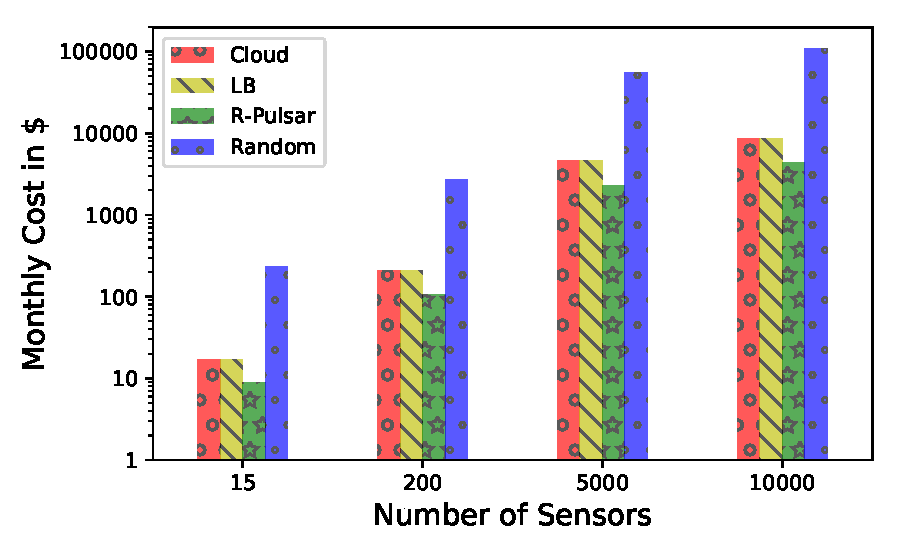
\includegraphics[width=0.8\textwidth]{Results/Cost_Amazon.pdf}
  \caption{Messaging cost savings evaluation based on the Amazon IoT pricing model, for four different setups.}
  \label{fig:cost-amazon}
\end{figure} 


Figure~\ref{fig:cost-amazon} depicts the cost of deploying the ETL dataflow using the Amazon cost model. Our system obtains a 50\% cost reduction when compared to the cloud and LB approaches in all four different setups (15, 200, 5000 and 10000 sensors). In addition our system obtains a 97\% savings when compared to the Random approach in all four different setups.

\begin{figure}[h]
  \centering
  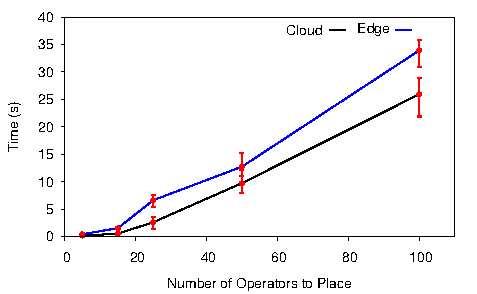
\includegraphics[width=0.8\textwidth]{Results/Scale.pdf}
  \caption{Evaluation of the scalability of the operator placement problem algorithm as the number of operators to place increase over edge and cloud resources.}\label{fig:scalefirst}
\end{figure}

Figure~\ref{fig:scalefirst} depicts the scalability and the overhead of the initial operator placement problem algorithm in both edge and cloud resources. We can observe that the algorithm scales with the number of operators to place and a valid solution can be found in less than half a minute.

\begin{figure}[h]
  \centering
  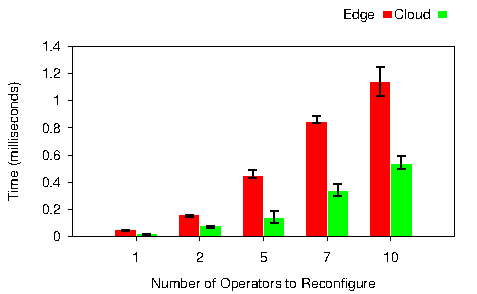
\includegraphics[width=0.8\textwidth]{Results/Redeploy.pdf}
  \caption{Evaluation of the cost of redeploying a subset of operators over edge and cloud resources.}\label{fig:scalesecond}
\end{figure}

Figure~\ref{fig:scalefirst} depicts the redeployment scalability and overhead of the algorithm. We can observer that since we do not need to redeploy all the operators when the workflow is not meeting the constraints, we can see that the cost of redeploying a subset of operators is very low and more important decisions can be done in real time since it the redeployment calculations are small.

\begin{figure}[h]
  \centering
  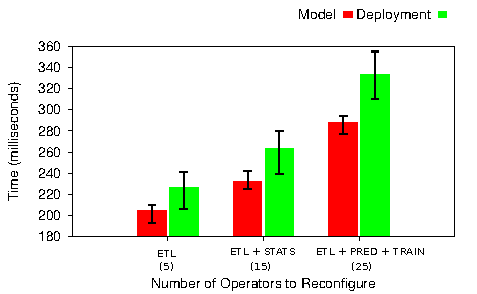
\includegraphics[width=0.8\textwidth]{Results/Time.pdf}
  \caption{Evaluation of the real-time vs the modeled time as the number of operators increases.}\label{fig:validation} 
\end{figure}

The final result we wanted to validate the model by comparing the expected results and the actual results after deploying the workflow in a real setup, Figure~\ref{fig:validation} depicts the results. We can observe that when the number of operators is small the difference between the expected and the actual results only differs by at most 10\%, when the number of operators grows to 25 the difference slightly grows up to 15\%.
